% !TeX program = xelatex
% 黑白論文版；將兩張 PDF 上傳到學姐專案的 figsrc/ch02/。
% 分別將下列段落插入 2.4 節開頭與 2.4.1。
% 不包含 chapter 或 section，不需另外設定圖號。
% 本檔與「第二章_插圖片段.tex」內容相同，擇一使用。

% 2.4 節開頭：放在介紹整體系統資訊流的段落之後。
本研究之整體控制架構設計如\cref{fig:system_control_architecture}所示。雷射感知提供障礙資訊，視覺量測與任務資訊則用於生成導航及操作參考，再由全身預測控制器共同求解底盤與手臂輸入。命令經各自之執行介面作用於移動機械臂，並將狀態與命令執行資訊回授至控制端。圖中實線表示量測、參考與命令的傳遞，虛線表示回授資訊。
\begin{figure}[htbp]
    \centering
    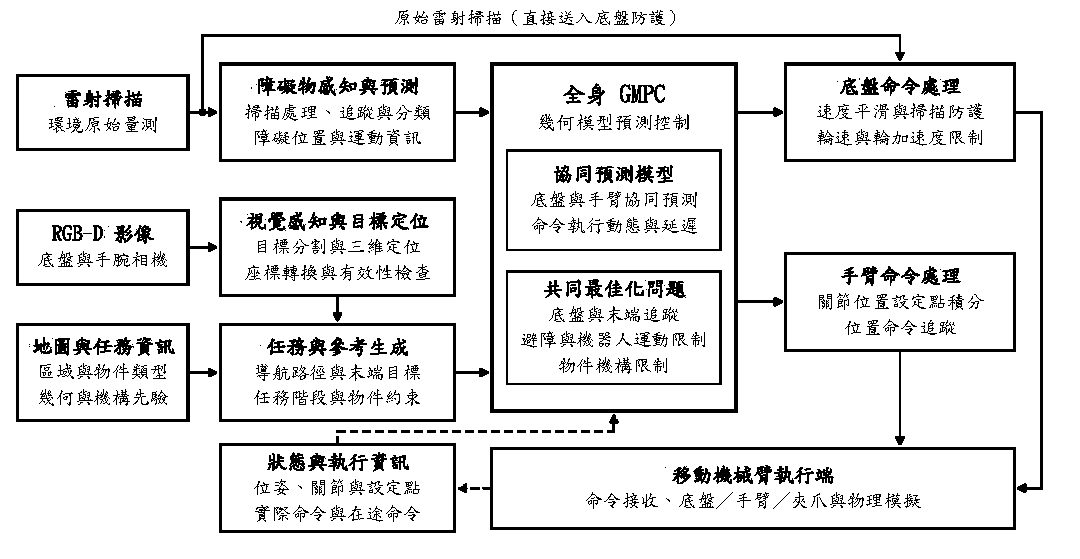
\includegraphics[width=1.0\textwidth]{figsrc/ch02/system_control_architecture.pdf}
    \caption{導航、視覺與操作之整體控制架構設計}
    \label{fig:system_control_architecture}
\end{figure}

% 2.4.1：放在說明導航參考與障礙資訊如何進入控制器的段落之後。
底盤導航架構如\cref{fig:navigation_architecture}所示。路徑規劃、障礙感知與定位資訊共同提供予 GMPC，預測式控制障壁函數（CBF）之避障條件則納入同一最佳化問題。控制器輸出依序經速度平滑器、近距離安全層與輪級命令限制器，形成最終底盤命令；原始雷射掃描另直接提供予安全層，底盤運動則透過里程計與定位模組形成閉迴路。
\begin{figure}[htbp]
    \centering
    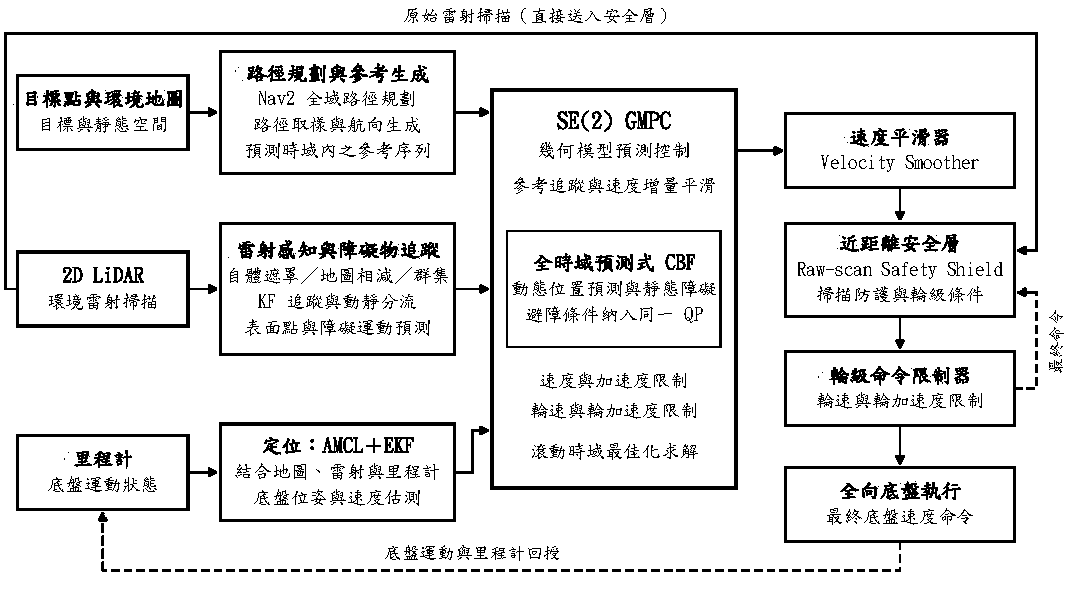
\includegraphics[width=1.0\textwidth]{figsrc/ch02/navigation_architecture.pdf}
    \caption{底盤幾何模型預測導航架構}
    \label{fig:navigation_architecture}
\end{figure}
